\section{Introduction to Operating Systems}

\subsection{Basic Principles of Operating Systems}

\mult{2}

\begin{definition}{Operating System (OS)}\\
    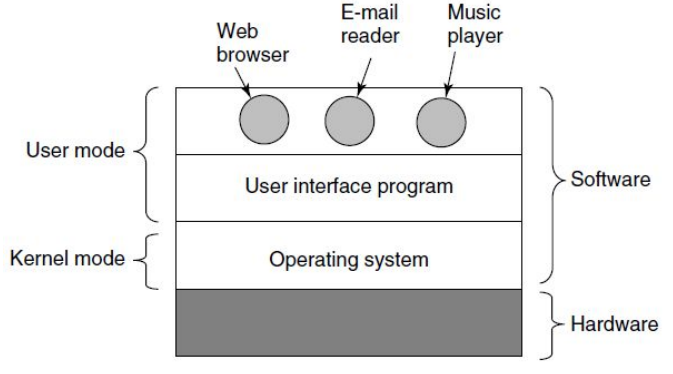
\includegraphics[width=\linewidth]{OS_def.png}
\end{definition}

\begin{theorem}{User Mode vs Kernel Mode}\\
    OS operate in two fundamental modes:
    \begin{itemize}
        \item \textbf{Kernel Mode}: Privileged execution mode with full access to all hardware resources and instructions
        \item \textbf{User Mode}: Restricted execution mode where applications run with limited privileges
    \end{itemize}
    
    The OS provides two key interfaces:
    \begin{itemize}
        \item \textbf{Northbound Interface}: User Interface \\ Towards user applications
        \item \textbf{Southbound Interface}: Hardware Interface \\ Towards hardware
    \end{itemize}
\end{theorem}

\multend

\mult{2}

\begin{concept}{The Operating System as an Extended Machine}\\
    The operating system serves as an abstraction layer between hardware and applications (software that manages hardware)
    \begin{itemize}
        \item Hardware: complex/difficult to program directly
        \item OSs create good abstractions for hardware resources (provide services for programs)
        \item These abstractions are implemented and \\ managed by the OS
        \item Provide services for programs: \\ Applications interact with these abstractions rather than directly with hardware
    \end{itemize}
    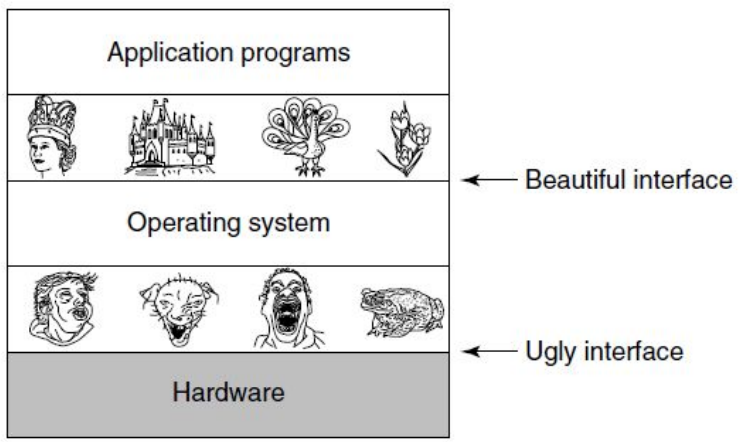
\includegraphics[width=\linewidth]{OS_overview.png}
\end{concept}

\begin{concept}{The Operating System as a Resource Manager}
    \begin{itemize}
        \item Process Management
        \item Memory Management
        \item File System Management
        \item Device Management
        \item Security
    \end{itemize}
    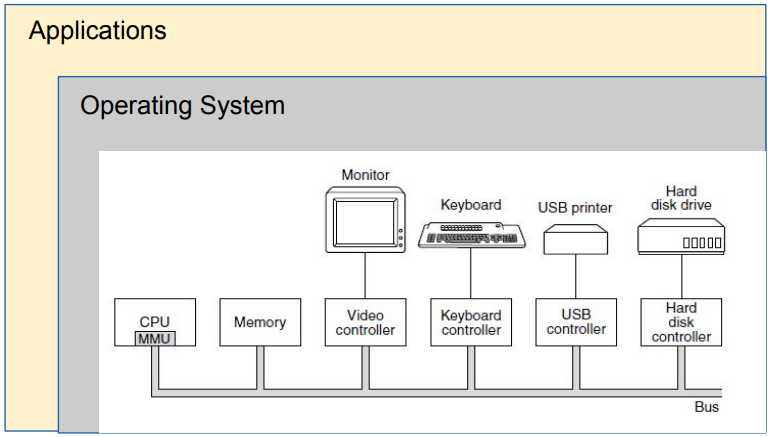
\includegraphics[width=\linewidth]{os_resource_magaer.png}
    \begin{itemize}
        \item Controls resource usage
        \item Grants resource requests
        \item Accounts for resource usage
        \item Mediates conflicting requests
        \item Ensures fair and efficient resource allocation
    \end{itemize}
\end{concept}

\multend

\raggedcolumns

\subsection{Operating System Variants}

\mult{2}

\begin{theorem}{Operating System Variants}
    \begin{itemize}
        \item Mainframe OS: IBM z/OS, IBM z/VM
        \item Server OS: Windows Server, Linux, Solaris
        \item Multiprocessor OS: Windows, Linux, Solaris
        \item Personal Computer OS: Windows, MacOS, Linux
        \item Handheld Computer OS: Android, iOS
        \item Embedded OS: VxWorks, QNX
        \item Real-Time OS: VxWorks, QNX
        \item Sensor Node OS: TinyOS, Contiki
        \item Cloud OS: OpenStack, OpenNebula
        \item Smart Card OS: JavaCard, MULTOS
    \end{itemize}
\end{theorem}

\begin{corollary}{Operating Systems vs. Distributions}
    \begin{itemize}
        \item \textbf{Operating System (Kernel)}: The core component that directly manages hardware resources
        \item \textbf{Distribution}: A complete package including kernel, utilities, and applications
    \end{itemize}
    Example: \\Linux Kernel + GNU Tools + X11 + Gnome \\ + Firefox + LibreOffice \\ = Ubuntu
\end{corollary}

\multend

\subsection{Basic OS Concepts}

\begin{definition}{Fundamental OS Concepts}
    \begin{itemize}
        \item \textbf{Interacting with OS}: Through terminal or graphical user interface
        \item \textbf{Users}: Regular vs. privileged users
        \item \textbf{Data organization}: Files, directories, filesystems
        \item \textbf{Programs vs. Processes}: A program is a compiled executable, while a process is an instance of a running program
        \item \textbf{Multi-tasking}: Running multiple processes concurrently
        \item \textbf{Context-switching}: Switching execution from one process to another
        \item \textbf{System calls}: Interface for processes to request OS services
        \item \textbf{Inter-Process Communication}: Methods for processes to communicate
        \item \textbf{Signals}: Mechanism for notifying processes of events
    \end{itemize}
\end{definition}

\begin{definition}{OS Structures}\\
    Operating systems can be organized in different ways:
    \begin{itemize}
        \item \textbf{Monolithic Systems}: Single executable containing all OS functionality
        \item \textbf{Modular Systems}: Core kernel with loadable modules
        \item \textbf{Microkernels}: Minimal kernel with most services running in user space
    \end{itemize}
\end{definition}

\begin{example}
    To check CPU information in Linux:
    \begin{lstlisting}[language=bash, style=basesmol]
    # Display kernel version information
    uname -a
    
    # View CPU details
    less /proc/cpuinfo
    
    # Display CPU architecture information
    lscpu
    \end{lstlisting}
\end{example}

\begin{KR}{Working with Processes in Linux}
    \paragraph{Viewing running processes}
    \begin{itemize}
        \item Use \texttt{ps aux} to display all processes
        \item Use \texttt{top} for an interactive process viewer
        \item Check environment variables with \texttt{env}
    \end{itemize}
    
    \paragraph{Process control}
    \begin{itemize}
        \item Background a process with \texttt{\&} or \texttt{bg}
        \item Bring to foreground with \texttt{fg}
        \item List background jobs with \texttt{jobs}
        \item Terminate a process with \texttt{kill PID}
    \end{itemize}
    
    \paragraph{System information}
    \begin{itemize}
        \item View process hierarchy with \texttt{pstree}
        \item Check system call activity with \texttt{strace}
    \end{itemize}
\end{KR}

\columnbreak

\subsection{Computer Hardware Review}

\subsubsection{CPU and Memory Architecture}

\begin{definition}{CPU} Central Processing Unit
    \begin{itemize}
        \item Basic cycle: Fetch, Decode, Execute
        \item CPUs feature some registers to hold key variables and temporary results
        \item Special registers for internal use: Program Counter (PC), Stack Pointer (SP), Program Status Word (PSW)
        \item Execution units and pipelines for processing instructions
        \item Cache memory organized in hierarchical levels (L1, L2, L3)
    \end{itemize}
    \vspace{1mm}
    CPUs and their Instruction Sets are architecture-specific:
    \begin{itemize}
        \item ARM, RISC, X86, etc.
        \item Instructions are classified along Execution Privileges, enforced by CPU:
        \begin{itemize}
            \item Intel: Priority Rings $\rightarrow$ User Mode (limited set of instructions) vs Kernel Mode (full set of instructions)
            \item ARM: UnPrivileged Mode vs Privileged Mode
        \end{itemize}
    \end{itemize}
\end{definition}



\begin{concept}{CPU cycles}

    \begin{minipage}{0.6\linewidth}
    Basic cycle of every CPU:    
    \begin{itemize}
        \item Fetch instructions from memory into registers
        \item Decode the instruction to determine type and operands
        \item Execute the instruction
        \item Repeat for subsequent instructions
    \end{itemize}
    CPUs have multiple cores:\\
    each having multiple execution units and parallel pipelines
    \end{minipage}
    \begin{minipage}{0.35\linewidth}
    \vspace{-5mm}
    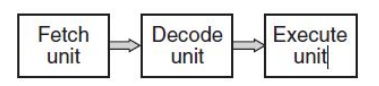
\includegraphics[width=0.7\linewidth]{cpu_cycles1.png}\\
    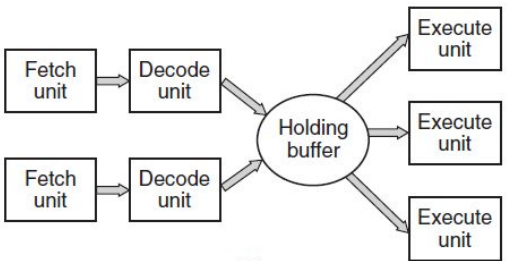
\includegraphics[width=\linewidth]{cpu_cycles2.png}
    \end{minipage}
\end{concept}

\begin{definition}{Memory}
    The memory system is constructed as a hierarchy of layers, based on access time:

    \begin{minipage}{0.4\linewidth}
    \begin{itemize}
        \item Registers (fastest, smallest)
        \item Cache memory (L1, L2, L3)
        \item Main memory (RAM)
        \item Secondary storage (disks, SSDs)
        \item Tertiary storage (backup systems)
    \end{itemize}
    \end{minipage}
    \begin{minipage}{0.59\linewidth}
    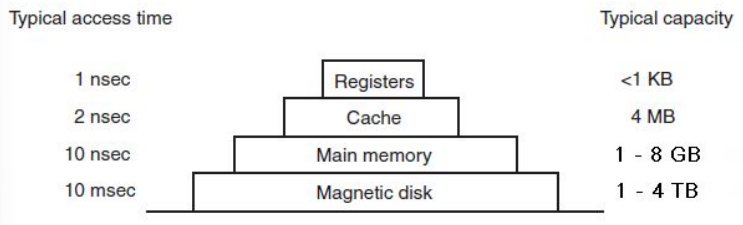
\includegraphics[width=\linewidth]{hardware_review_memory.png}
    \end{minipage}
\end{definition}

\begin{theorem}{CPU Caches} multiple levels of caches:

    \begin{minipage}{0.6\linewidth}
    \begin{itemize}
        \item L1: Small, fast, close to CPU
        \item L2: Larger, slower, further away
        \item L3: Even larger, even slower, even further away
        \item Caches are used to store frequently accessed data and instructions
    \end{itemize}    
    Example: Quad-core chip with shared L2 cache and quad-core chip with separate L2 caches for each core.
    \end{minipage}
    \begin{minipage}{0.39\linewidth}
    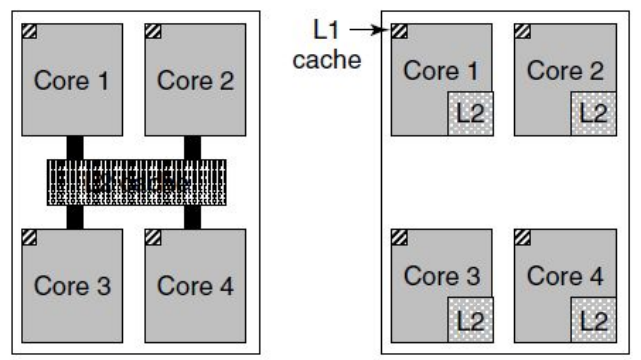
\includegraphics[width=\linewidth]{cpu_caches.png}    
    \end{minipage}
\end{theorem}

\columnbreak

\subsubsection{I/O System}

\mult{2}

\begin{definition}{Input/Output (I/O) System}\\
    The I/O system comprises:
    \begin{itemize}
        \item Various devices (hard drives, network interfaces, serial ports, keyboards, etc.)
        \item Bus systems to connect devices (PCI, PCIe, SATA, USB, etc.) (software)
        \item I/O controllers (hardware)
        \item Device drivers (software)
    \end{itemize}
    Device drivers:
    \begin{itemize}
        \item Software that communicates with I/O controllers (commands/responses)
        \item Can run in Kernel or User Mode
        \item May be built into the kernel or modular (loaded as modules at boot/run time)
    \end{itemize}
    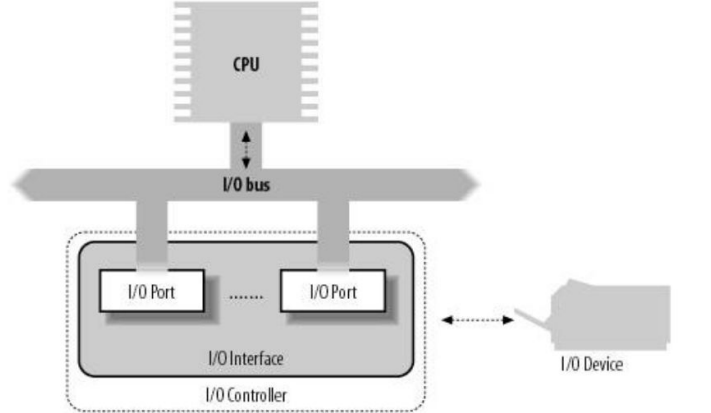
\includegraphics[width=\linewidth]{io_overview.png}
\end{definition}

\begin{example2}{IO and Bus System} X86 System with different Bus standards:

    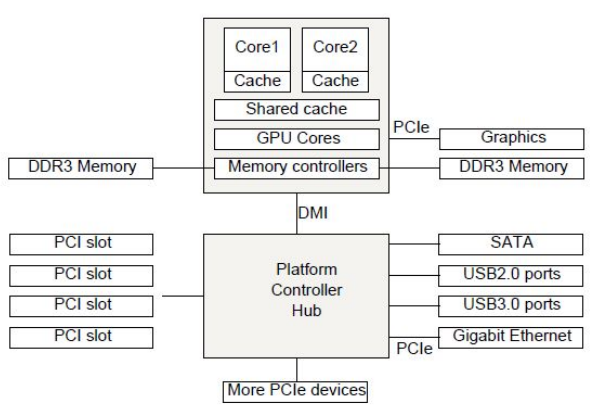
\includegraphics[width=\linewidth]{io_and_bus_syste_example.png}
\end{example2}

\multend





